\section{Análisis de Participación}
  % Graphic for TeX using PGF
% Title: /home/jnicolaschc/GitHub/Metodología de la Investigación/enfoque_marco_logico/Esquemas/Árbol de Participación/arbolParticipacion.dia
% Creator: Dia v0.97+git
% CreationDate: Sun Jun 27 19:22:05 2021
% For: jnicolaschc
% \usepackage{tikz}
% The following commands are not supported in PSTricks at present
% We define them conditionally, so when they are implemented,
% this pgf file will use them.
\begin{figure}[H]
    \centering
    \ifx\du\undefined
      \newlength{\du}
    \fi
    \setlength{\du}{15\unitlength}
    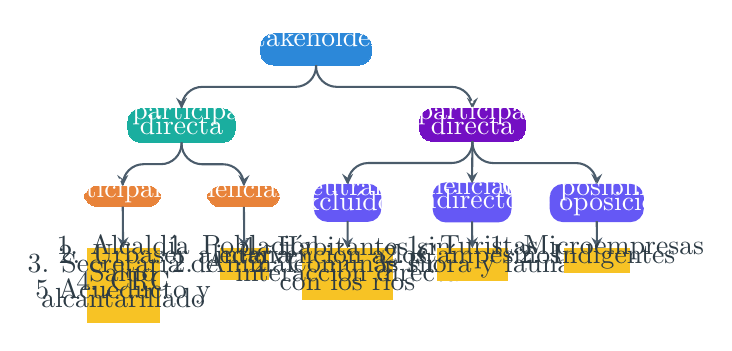
\begin{tikzpicture}[even odd rule]
    \pgftransformxscale{1.000000}
    \pgftransformyscale{-1.000000}
    \definecolor{dialinecolor}{rgb}{0.000000, 0.000000, 0.000000}
    \pgfsetstrokecolor{dialinecolor}
    \pgfsetstrokeopacity{1.000000}
    \definecolor{diafillcolor}{rgb}{1.000000, 1.000000, 1.000000}
    \pgfsetfillcolor{diafillcolor}
    \pgfsetfillopacity{1.000000}
    \pgfsetlinewidth{0.000000\du}
    \pgfsetdash{}{0pt}
    \pgfsetroundjoin
    \pgfsetbuttcap
    {\pgfsetcornersarced{\pgfpoint{0.300000\du}{0.300000\du}}\definecolor{diafillcolor}{rgb}{0.172549, 0.533333, 0.850980}
    \pgfsetfillcolor{diafillcolor}
    \pgfsetfillopacity{1.000000}
    \fill (49.907800\du,8.337130\du)--(49.907800\du,9.087734\du)--(52.579713\du,9.087734\du)--(52.579713\du,8.337130\du)--cycle;
    }{\pgfsetcornersarced{\pgfpoint{0.300000\du}{0.300000\du}}\definecolor{dialinecolor}{rgb}{0.172549, 0.533333, 0.850980}
    \pgfsetstrokecolor{dialinecolor}
    \pgfsetstrokeopacity{1.000000}
    \draw (49.907800\du,8.337130\du)--(49.907800\du,9.087734\du)--(52.579713\du,9.087734\du)--(52.579713\du,8.337130\du)--cycle;
    }% setfont left to latex
    \definecolor{dialinecolor}{rgb}{1.000000, 1.000000, 1.000000}
    \pgfsetstrokecolor{dialinecolor}
    \pgfsetstrokeopacity{1.000000}
    \definecolor{diafillcolor}{rgb}{1.000000, 1.000000, 1.000000}
    \pgfsetfillcolor{diafillcolor}
    \pgfsetfillopacity{1.000000}
    \node[anchor=base,inner sep=0pt, outer sep=0pt,color=dialinecolor] at (51.243800\du,8.651505\du){Stakeholders};
    \pgfsetlinewidth{0.000000\du}
    \pgfsetdash{}{0pt}
    \pgfsetroundjoin
    \pgfsetbuttcap
    {\pgfsetcornersarced{\pgfpoint{0.300000\du}{0.300000\du}}\definecolor{diafillcolor}{rgb}{0.450980, 0.058824, 0.764706}
    \pgfsetfillcolor{diafillcolor}
    \pgfsetfillopacity{1.000000}
    \fill (53.735000\du,10.140900\du)--(53.735000\du,10.923575\du)--(56.285803\du,10.923575\du)--(56.285803\du,10.140900\du)--cycle;
    }{\pgfsetcornersarced{\pgfpoint{0.300000\du}{0.300000\du}}\definecolor{dialinecolor}{rgb}{0.450980, 0.058824, 0.764706}
    \pgfsetstrokecolor{dialinecolor}
    \pgfsetstrokeopacity{1.000000}
    \draw (53.735000\du,10.140900\du)--(53.735000\du,10.923575\du)--(56.285803\du,10.923575\du)--(56.285803\du,10.140900\du)--cycle;
    }\pgfsetlinewidth{0.050000\du}
    \pgfsetdash{}{0pt}
    \pgfsetmiterjoin
    \pgfsetbuttcap
    {
    \definecolor{diafillcolor}{rgb}{0.294118, 0.360784, 0.419608}
    \pgfsetfillcolor{diafillcolor}
    \pgfsetfillopacity{1.000000}
    % was here!!!
    \pgfsetarrowsend{stealth}
    {\pgfsetcornersarced{\pgfpoint{0.500000\du}{0.500000\du}}\definecolor{dialinecolor}{rgb}{0.294118, 0.360784, 0.419608}
    \pgfsetstrokecolor{dialinecolor}
    \pgfsetstrokeopacity{1.000000}
    \draw (51.243756\du,9.087734\du)--(51.243756\du,9.614317\du)--(55.010402\du,9.614317\du)--(55.010402\du,10.140900\du);
    }}
    % setfont left to latex
    \definecolor{dialinecolor}{rgb}{1.000000, 1.000000, 1.000000}
    \pgfsetstrokecolor{dialinecolor}
    \pgfsetstrokeopacity{1.000000}
    \definecolor{diafillcolor}{rgb}{1.000000, 1.000000, 1.000000}
    \pgfsetfillcolor{diafillcolor}
    \pgfsetfillopacity{1.000000}
    \node[anchor=base,inner sep=0pt, outer sep=0pt,color=dialinecolor] at (55.010400\du,10.402853\du){Sin participación};
    % setfont left to latex
    \definecolor{dialinecolor}{rgb}{1.000000, 1.000000, 1.000000}
    \pgfsetstrokecolor{dialinecolor}
    \pgfsetstrokeopacity{1.000000}
    \definecolor{diafillcolor}{rgb}{1.000000, 1.000000, 1.000000}
    \pgfsetfillcolor{diafillcolor}
    \pgfsetfillopacity{1.000000}
    \node[anchor=base,inner sep=0pt, outer sep=0pt,color=dialinecolor] at (55.010400\du,10.755631\du){directa};
    \pgfsetlinewidth{0.000000\du}
    \pgfsetdash{}{0pt}
    \pgfsetroundjoin
    \pgfsetbuttcap
    {\pgfsetcornersarced{\pgfpoint{0.300000\du}{0.300000\du}}\definecolor{diafillcolor}{rgb}{0.101961, 0.682353, 0.623529}
    \pgfsetfillcolor{diafillcolor}
    \pgfsetfillopacity{1.000000}
    \fill (46.713200\du,10.140900\du)--(46.713200\du,10.951096\du)--(49.293356\du,10.951096\du)--(49.293356\du,10.140900\du)--cycle;
    }{\pgfsetcornersarced{\pgfpoint{0.300000\du}{0.300000\du}}\definecolor{dialinecolor}{rgb}{0.101961, 0.682353, 0.623529}
    \pgfsetstrokecolor{dialinecolor}
    \pgfsetstrokeopacity{1.000000}
    \draw (46.713200\du,10.140900\du)--(46.713200\du,10.951096\du)--(49.293356\du,10.951096\du)--(49.293356\du,10.140900\du)--cycle;
    }% setfont left to latex
    \definecolor{dialinecolor}{rgb}{1.000000, 1.000000, 1.000000}
    \pgfsetstrokecolor{dialinecolor}
    \pgfsetstrokeopacity{1.000000}
    \definecolor{diafillcolor}{rgb}{1.000000, 1.000000, 1.000000}
    \pgfsetfillcolor{diafillcolor}
    \pgfsetfillopacity{1.000000}
    \node[anchor=base,inner sep=0pt, outer sep=0pt,color=dialinecolor] at (48.003300\du,10.402853\du){Con participación};
    % setfont left to latex
    \definecolor{dialinecolor}{rgb}{1.000000, 1.000000, 1.000000}
    \pgfsetstrokecolor{dialinecolor}
    \pgfsetstrokeopacity{1.000000}
    \definecolor{diafillcolor}{rgb}{1.000000, 1.000000, 1.000000}
    \pgfsetfillcolor{diafillcolor}
    \pgfsetfillopacity{1.000000}
    \node[anchor=base,inner sep=0pt, outer sep=0pt,color=dialinecolor] at (48.003300\du,10.755631\du){directa};
    \pgfsetlinewidth{0.050000\du}
    \pgfsetdash{}{0pt}
    \pgfsetmiterjoin
    \pgfsetbuttcap
    {
    \definecolor{diafillcolor}{rgb}{0.294118, 0.360784, 0.419608}
    \pgfsetfillcolor{diafillcolor}
    \pgfsetfillopacity{1.000000}
    % was here!!!
    \pgfsetarrowsend{stealth}
    {\pgfsetcornersarced{\pgfpoint{0.500000\du}{0.500000\du}}\definecolor{dialinecolor}{rgb}{0.294118, 0.360784, 0.419608}
    \pgfsetstrokecolor{dialinecolor}
    \pgfsetstrokeopacity{1.000000}
    \draw (51.243756\du,9.087734\du)--(51.243756\du,9.614317\du)--(48.003278\du,9.614317\du)--(48.003278\du,10.140900\du);
    }}
    \pgfsetlinewidth{0.050000\du}
    \pgfsetdash{}{0pt}
    \pgfsetmiterjoin
    \pgfsetbuttcap
    {
    \definecolor{diafillcolor}{rgb}{0.294118, 0.360784, 0.419608}
    \pgfsetfillcolor{diafillcolor}
    \pgfsetfillopacity{1.000000}
    % was here!!!
    \pgfsetarrowsend{stealth}
    {\pgfsetcornersarced{\pgfpoint{0.500000\du}{0.500000\du}}\definecolor{dialinecolor}{rgb}{0.294118, 0.360784, 0.419608}
    \pgfsetstrokecolor{dialinecolor}
    \pgfsetstrokeopacity{1.000000}
    \draw (48.003278\du,10.951096\du)--(48.003278\du,11.478898\du)--(49.505825\du,11.478898\du)--(49.505825\du,12.006700\du);
    }}
    \pgfsetlinewidth{0.050000\du}
    \pgfsetdash{}{0pt}
    \pgfsetmiterjoin
    \pgfsetbuttcap
    {
    \definecolor{diafillcolor}{rgb}{0.294118, 0.360784, 0.419608}
    \pgfsetfillcolor{diafillcolor}
    \pgfsetfillopacity{1.000000}
    % was here!!!
    \pgfsetarrowsend{stealth}
    {\pgfsetcornersarced{\pgfpoint{0.500000\du}{0.500000\du}}\definecolor{dialinecolor}{rgb}{0.294118, 0.360784, 0.419608}
    \pgfsetstrokecolor{dialinecolor}
    \pgfsetstrokeopacity{1.000000}
    \draw (48.003278\du,10.951096\du)--(48.003278\du,11.477048\du)--(46.586887\du,11.477048\du)--(46.586887\du,12.003000\du);
    }}
    \pgfsetlinewidth{0.000000\du}
    \pgfsetdash{}{0pt}
    \pgfsetroundjoin
    \pgfsetbuttcap
    {\pgfsetcornersarced{\pgfpoint{0.300000\du}{0.300000\du}}\definecolor{diafillcolor}{rgb}{0.909804, 0.513726, 0.227451}
    \pgfsetfillcolor{diafillcolor}
    \pgfsetfillopacity{1.000000}
    \fill (45.677300\du,12.003000\du)--(45.677300\du,12.499266\du)--(47.496475\du,12.499266\du)--(47.496475\du,12.003000\du)--cycle;
    }{\pgfsetcornersarced{\pgfpoint{0.300000\du}{0.300000\du}}\definecolor{dialinecolor}{rgb}{0.909804, 0.513726, 0.227451}
    \pgfsetstrokecolor{dialinecolor}
    \pgfsetstrokeopacity{1.000000}
    \draw (45.677300\du,12.003000\du)--(45.677300\du,12.499266\du)--(47.496475\du,12.499266\du)--(47.496475\du,12.003000\du)--cycle;
    }\pgfsetlinewidth{0.000000\du}
    \pgfsetdash{}{0pt}
    \pgfsetroundjoin
    \pgfsetbuttcap
    {\pgfsetcornersarced{\pgfpoint{0.300000\du}{0.300000\du}}\definecolor{diafillcolor}{rgb}{0.909804, 0.513726, 0.227451}
    \pgfsetfillcolor{diafillcolor}
    \pgfsetfillopacity{1.000000}
    \fill (48.639800\du,12.006700\du)--(48.639800\du,12.506698\du)--(50.371850\du,12.506698\du)--(50.371850\du,12.006700\du)--cycle;
    }{\pgfsetcornersarced{\pgfpoint{0.300000\du}{0.300000\du}}\definecolor{dialinecolor}{rgb}{0.909804, 0.513726, 0.227451}
    \pgfsetstrokecolor{dialinecolor}
    \pgfsetstrokeopacity{1.000000}
    \draw (48.639800\du,12.006700\du)--(48.639800\du,12.506698\du)--(50.371850\du,12.506698\du)--(50.371850\du,12.006700\du)--cycle;
    }% setfont left to latex
    \definecolor{dialinecolor}{rgb}{1.000000, 1.000000, 1.000000}
    \pgfsetstrokecolor{dialinecolor}
    \pgfsetstrokeopacity{1.000000}
    \definecolor{diafillcolor}{rgb}{1.000000, 1.000000, 1.000000}
    \pgfsetfillcolor{diafillcolor}
    \pgfsetfillopacity{1.000000}
    \node[anchor=base,inner sep=0pt, outer sep=0pt,color=dialinecolor] at (46.586900\du,12.272353\du){Participantes};
    % setfont left to latex
    \definecolor{dialinecolor}{rgb}{1.000000, 1.000000, 1.000000}
    \pgfsetstrokecolor{dialinecolor}
    \pgfsetstrokeopacity{1.000000}
    \definecolor{diafillcolor}{rgb}{1.000000, 1.000000, 1.000000}
    \pgfsetfillcolor{diafillcolor}
    \pgfsetfillopacity{1.000000}
    \node[anchor=base,inner sep=0pt, outer sep=0pt,color=dialinecolor] at (49.505800\du,12.268653\du){Beneficiarios};
    \pgfsetlinewidth{0.050000\du}
    \pgfsetdash{}{0pt}
    \pgfsetmiterjoin
    \pgfsetbuttcap
    {
    \definecolor{diafillcolor}{rgb}{0.294118, 0.360784, 0.419608}
    \pgfsetfillcolor{diafillcolor}
    \pgfsetfillopacity{1.000000}
    % was here!!!
    \pgfsetarrowsend{stealth}
    {\pgfsetcornersarced{\pgfpoint{0.500000\du}{0.500000\du}}\definecolor{dialinecolor}{rgb}{0.294118, 0.360784, 0.419608}
    \pgfsetstrokecolor{dialinecolor}
    \pgfsetstrokeopacity{1.000000}
    \draw (55.010402\du,10.923575\du)--(55.010402\du,11.449837\du)--(58.005318\du,11.449837\du)--(58.005318\du,11.976100\du);
    }}
    \pgfsetlinewidth{0.050000\du}
    \pgfsetdash{}{0pt}
    \pgfsetmiterjoin
    \pgfsetbuttcap
    {
    \definecolor{diafillcolor}{rgb}{0.294118, 0.360784, 0.419608}
    \pgfsetfillcolor{diafillcolor}
    \pgfsetfillopacity{1.000000}
    % was here!!!
    \pgfsetarrowsend{stealth}
    {\pgfsetcornersarced{\pgfpoint{0.500000\du}{0.500000\du}}\definecolor{dialinecolor}{rgb}{0.294118, 0.360784, 0.419608}
    \pgfsetstrokecolor{dialinecolor}
    \pgfsetstrokeopacity{1.000000}
    \draw (55.010402\du,10.923575\du)--(55.010402\du,11.448587\du)--(52.003848\du,11.448587\du)--(52.003848\du,11.973600\du);
    }}
    \pgfsetlinewidth{0.050000\du}
    \pgfsetdash{}{0pt}
    \pgfsetroundjoin
    \pgfsetbuttcap
    {\pgfsetcornersarced{\pgfpoint{0.300000\du}{0.300000\du}}\definecolor{diafillcolor}{rgb}{0.396078, 0.345098, 0.960784}
    \pgfsetfillcolor{diafillcolor}
    \pgfsetfillopacity{1.000000}
    \fill (51.214800\du,11.973600\du)--(51.214800\du,12.840258\du)--(52.792896\du,12.840258\du)--(52.792896\du,11.973600\du)--cycle;
    }{\pgfsetcornersarced{\pgfpoint{0.300000\du}{0.300000\du}}\definecolor{dialinecolor}{rgb}{0.396078, 0.345098, 0.960784}
    \pgfsetstrokecolor{dialinecolor}
    \pgfsetstrokeopacity{1.000000}
    \draw (51.214800\du,11.973600\du)--(51.214800\du,12.840258\du)--(52.792896\du,12.840258\du)--(52.792896\du,11.973600\du)--cycle;
    }\pgfsetlinewidth{0.050000\du}
    \pgfsetdash{}{0pt}
    \pgfsetroundjoin
    \pgfsetbuttcap
    {\pgfsetcornersarced{\pgfpoint{0.300000\du}{0.300000\du}}\definecolor{diafillcolor}{rgb}{0.396078, 0.345098, 0.960784}
    \pgfsetfillcolor{diafillcolor}
    \pgfsetfillopacity{1.000000}
    \fill (56.896000\du,11.976100\du)--(56.896000\du,12.848566\du)--(59.114637\du,12.848566\du)--(59.114637\du,11.976100\du)--cycle;
    }{\pgfsetcornersarced{\pgfpoint{0.300000\du}{0.300000\du}}\definecolor{dialinecolor}{rgb}{0.396078, 0.345098, 0.960784}
    \pgfsetstrokecolor{dialinecolor}
    \pgfsetstrokeopacity{1.000000}
    \draw (56.896000\du,11.976100\du)--(56.896000\du,12.848566\du)--(59.114637\du,12.848566\du)--(59.114637\du,11.976100\du)--cycle;
    }\pgfsetlinewidth{0.050000\du}
    \pgfsetdash{}{0pt}
    \pgfsetroundjoin
    \pgfsetbuttcap
    {\pgfsetcornersarced{\pgfpoint{0.300000\du}{0.300000\du}}\definecolor{diafillcolor}{rgb}{0.396078, 0.345098, 0.960784}
    \pgfsetfillcolor{diafillcolor}
    \pgfsetfillopacity{1.000000}
    \fill (54.077300\du,11.938300\du)--(54.077300\du,12.856026\du)--(55.926869\du,12.856026\du)--(55.926869\du,11.938300\du)--cycle;
    }{\pgfsetcornersarced{\pgfpoint{0.300000\du}{0.300000\du}}\definecolor{dialinecolor}{rgb}{0.396078, 0.345098, 0.960784}
    \pgfsetstrokecolor{dialinecolor}
    \pgfsetstrokeopacity{1.000000}
    \draw (54.077300\du,11.938300\du)--(54.077300\du,12.856026\du)--(55.926869\du,12.856026\du)--(55.926869\du,11.938300\du)--cycle;
    }\pgfsetlinewidth{0.050000\du}
    \pgfsetdash{}{0pt}
    \pgfsetbuttcap
    {
    \definecolor{diafillcolor}{rgb}{0.294118, 0.360784, 0.419608}
    \pgfsetfillcolor{diafillcolor}
    \pgfsetfillopacity{1.000000}
    % was here!!!
    \pgfsetarrowsend{stealth}
    \definecolor{dialinecolor}{rgb}{0.294118, 0.360784, 0.419608}
    \pgfsetstrokecolor{dialinecolor}
    \pgfsetstrokeopacity{1.000000}
    \draw (55.010400\du,10.923600\du)--(55.002100\du,11.938300\du);
    }
    % setfont left to latex
    \definecolor{dialinecolor}{rgb}{1.000000, 1.000000, 1.000000}
    \pgfsetstrokecolor{dialinecolor}
    \pgfsetstrokeopacity{1.000000}
    \definecolor{diafillcolor}{rgb}{1.000000, 1.000000, 1.000000}
    \pgfsetfillcolor{diafillcolor}
    \pgfsetfillopacity{1.000000}
    \node[anchor=base,inner sep=0pt, outer sep=0pt,color=dialinecolor] at (52.003800\du,12.235553\du){Neutrales};
    % setfont left to latex
    \definecolor{dialinecolor}{rgb}{1.000000, 1.000000, 1.000000}
    \pgfsetstrokecolor{dialinecolor}
    \pgfsetstrokeopacity{1.000000}
    \definecolor{diafillcolor}{rgb}{1.000000, 1.000000, 1.000000}
    \pgfsetfillcolor{diafillcolor}
    \pgfsetfillopacity{1.000000}
    \node[anchor=base,inner sep=0pt, outer sep=0pt,color=dialinecolor] at (52.003800\du,12.588331\du){(excluídos)};
    % setfont left to latex
    \definecolor{dialinecolor}{rgb}{1.000000, 1.000000, 1.000000}
    \pgfsetstrokecolor{dialinecolor}
    \pgfsetstrokeopacity{1.000000}
    \definecolor{diafillcolor}{rgb}{1.000000, 1.000000, 1.000000}
    \pgfsetfillcolor{diafillcolor}
    \pgfsetfillopacity{1.000000}
    \node[anchor=base,inner sep=0pt, outer sep=0pt,color=dialinecolor] at (55.002100\du,12.200253\du){Beneficiarios};
    % setfont left to latex
    \definecolor{dialinecolor}{rgb}{1.000000, 1.000000, 1.000000}
    \pgfsetstrokecolor{dialinecolor}
    \pgfsetstrokeopacity{1.000000}
    \definecolor{diafillcolor}{rgb}{1.000000, 1.000000, 1.000000}
    \pgfsetfillcolor{diafillcolor}
    \pgfsetfillopacity{1.000000}
    \node[anchor=base,inner sep=0pt, outer sep=0pt,color=dialinecolor] at (55.002100\du,12.553031\du){indirectos};
    % setfont left to latex
    \definecolor{dialinecolor}{rgb}{1.000000, 1.000000, 1.000000}
    \pgfsetstrokecolor{dialinecolor}
    \pgfsetstrokeopacity{1.000000}
    \definecolor{diafillcolor}{rgb}{1.000000, 1.000000, 1.000000}
    \pgfsetfillcolor{diafillcolor}
    \pgfsetfillopacity{1.000000}
    \node[anchor=base,inner sep=0pt, outer sep=0pt,color=dialinecolor] at (58.005300\du,12.238053\du){Con posibilidad};
    % setfont left to latex
    \definecolor{dialinecolor}{rgb}{1.000000, 1.000000, 1.000000}
    \pgfsetstrokecolor{dialinecolor}
    \pgfsetstrokeopacity{1.000000}
    \definecolor{diafillcolor}{rgb}{1.000000, 1.000000, 1.000000}
    \pgfsetfillcolor{diafillcolor}
    \pgfsetfillopacity{1.000000}
    \node[anchor=base,inner sep=0pt, outer sep=0pt,color=dialinecolor] at (58.005300\du,12.590831\du){ de oposición};
    \pgfsetlinewidth{0.050000\du}
    \pgfsetdash{}{0pt}
    \pgfsetbuttcap
    {
    \definecolor{diafillcolor}{rgb}{0.294118, 0.360784, 0.419608}
    \pgfsetfillcolor{diafillcolor}
    \pgfsetfillopacity{1.000000}
    % was here!!!
    \pgfsetarrowsend{stealth}
    \definecolor{dialinecolor}{rgb}{0.294118, 0.360784, 0.419608}
    \pgfsetstrokecolor{dialinecolor}
    \pgfsetstrokeopacity{1.000000}
    \draw (46.586900\du,12.499300\du)--(46.595300\du,13.500100\du);
    }
    \pgfsetlinewidth{0.000000\du}
    \pgfsetdash{}{0pt}
    \pgfsetmiterjoin
    \pgfsetbuttcap
    {\pgfsetcornersarced{\pgfpoint{0.000000\du}{0.000000\du}}\definecolor{diafillcolor}{rgb}{0.968627, 0.764706, 0.145098}
    \pgfsetfillcolor{diafillcolor}
    \pgfsetfillopacity{1.000000}
    \fill (45.727300\du,13.500100\du)--(45.727300\du,15.295029\du)--(47.463306\du,15.295029\du)--(47.463306\du,13.500100\du)--cycle;
    }{\pgfsetcornersarced{\pgfpoint{0.000000\du}{0.000000\du}}\definecolor{dialinecolor}{rgb}{0.968627, 0.764706, 0.145098}
    \pgfsetstrokecolor{dialinecolor}
    \pgfsetstrokeopacity{1.000000}
    \draw (45.727300\du,13.500100\du)--(45.727300\du,15.295029\du)--(47.463306\du,15.295029\du)--(47.463306\du,13.500100\du)--cycle;
    }% setfont left to latex
    \definecolor{dialinecolor}{rgb}{0.176471, 0.231373, 0.270588}
    \pgfsetstrokecolor{dialinecolor}
    \pgfsetstrokeopacity{1.000000}
    \definecolor{diafillcolor}{rgb}{0.176471, 0.231373, 0.270588}
    \pgfsetfillcolor{diafillcolor}
    \pgfsetfillopacity{1.000000}
    \node[anchor=base,inner sep=0pt, outer sep=0pt,color=dialinecolor] at (46.595300\du,13.662215\du){1. Alcaldía};
    % setfont left to latex
    \definecolor{dialinecolor}{rgb}{0.176471, 0.231373, 0.270588}
    \pgfsetstrokecolor{dialinecolor}
    \pgfsetstrokeopacity{1.000000}
    \definecolor{diafillcolor}{rgb}{0.176471, 0.231373, 0.270588}
    \pgfsetfillcolor{diafillcolor}
    \pgfsetfillopacity{1.000000}
    \node[anchor=base,inner sep=0pt, outer sep=0pt,color=dialinecolor] at (46.595300\du,13.873882\du){2. Urbaser};
    % setfont left to latex
    \definecolor{dialinecolor}{rgb}{0.176471, 0.231373, 0.270588}
    \pgfsetstrokecolor{dialinecolor}
    \pgfsetstrokeopacity{1.000000}
    \definecolor{diafillcolor}{rgb}{0.176471, 0.231373, 0.270588}
    \pgfsetfillcolor{diafillcolor}
    \pgfsetfillopacity{1.000000}
    \node[anchor=base,inner sep=0pt, outer sep=0pt,color=dialinecolor] at (46.595300\du,14.085549\du){3. Secretaria de};
    % setfont left to latex
    \definecolor{dialinecolor}{rgb}{0.176471, 0.231373, 0.270588}
    \pgfsetstrokecolor{dialinecolor}
    \pgfsetstrokeopacity{1.000000}
    \definecolor{diafillcolor}{rgb}{0.176471, 0.231373, 0.270588}
    \pgfsetfillcolor{diafillcolor}
    \pgfsetfillopacity{1.000000}
    \node[anchor=base,inner sep=0pt, outer sep=0pt,color=dialinecolor] at (46.595300\du,14.297215\du){Salud};
    % setfont left to latex
    \definecolor{dialinecolor}{rgb}{0.176471, 0.231373, 0.270588}
    \pgfsetstrokecolor{dialinecolor}
    \pgfsetstrokeopacity{1.000000}
    \definecolor{diafillcolor}{rgb}{0.176471, 0.231373, 0.270588}
    \pgfsetfillcolor{diafillcolor}
    \pgfsetfillopacity{1.000000}
    \node[anchor=base,inner sep=0pt, outer sep=0pt,color=dialinecolor] at (46.595300\du,14.508882\du){4. CRC};
    % setfont left to latex
    \definecolor{dialinecolor}{rgb}{0.176471, 0.231373, 0.270588}
    \pgfsetstrokecolor{dialinecolor}
    \pgfsetstrokeopacity{1.000000}
    \definecolor{diafillcolor}{rgb}{0.176471, 0.231373, 0.270588}
    \pgfsetfillcolor{diafillcolor}
    \pgfsetfillopacity{1.000000}
    \node[anchor=base,inner sep=0pt, outer sep=0pt,color=dialinecolor] at (46.595300\du,14.720549\du){5 Acueducto y};
    % setfont left to latex
    \definecolor{dialinecolor}{rgb}{0.176471, 0.231373, 0.270588}
    \pgfsetstrokecolor{dialinecolor}
    \pgfsetstrokeopacity{1.000000}
    \definecolor{diafillcolor}{rgb}{0.176471, 0.231373, 0.270588}
    \pgfsetfillcolor{diafillcolor}
    \pgfsetfillopacity{1.000000}
    \node[anchor=base,inner sep=0pt, outer sep=0pt,color=dialinecolor] at (46.595300\du,14.932215\du){alcantarillado};
    \pgfsetlinewidth{0.050000\du}
    \pgfsetdash{}{0pt}
    \pgfsetbuttcap
    {
    \definecolor{diafillcolor}{rgb}{0.294118, 0.360784, 0.419608}
    \pgfsetfillcolor{diafillcolor}
    \pgfsetfillopacity{1.000000}
    % was here!!!
    \pgfsetarrowsend{stealth}
    \definecolor{dialinecolor}{rgb}{0.294118, 0.360784, 0.419608}
    \pgfsetstrokecolor{dialinecolor}
    \pgfsetstrokeopacity{1.000000}
    \draw (49.505800\du,12.506700\du)--(49.515100\du,13.506400\du);
    }
    \pgfsetlinewidth{0.000000\du}
    \pgfsetdash{}{0pt}
    \pgfsetmiterjoin
    \pgfsetbuttcap
    {\pgfsetcornersarced{\pgfpoint{0.000000\du}{0.000000\du}}\definecolor{diafillcolor}{rgb}{0.968627, 0.764706, 0.145098}
    \pgfsetfillcolor{diafillcolor}
    \pgfsetfillopacity{1.000000}
    \fill (48.939800\du,13.506400\du)--(48.939800\du,14.263161\du)--(50.090347\du,14.263161\du)--(50.090347\du,13.506400\du)--cycle;
    }{\pgfsetcornersarced{\pgfpoint{0.000000\du}{0.000000\du}}\definecolor{dialinecolor}{rgb}{0.968627, 0.764706, 0.145098}
    \pgfsetstrokecolor{dialinecolor}
    \pgfsetstrokeopacity{1.000000}
    \draw (48.939800\du,13.506400\du)--(48.939800\du,14.263161\du)--(50.090347\du,14.263161\du)--(50.090347\du,13.506400\du)--cycle;
    }% setfont left to latex
    \definecolor{dialinecolor}{rgb}{0.176471, 0.231373, 0.270588}
    \pgfsetstrokecolor{dialinecolor}
    \pgfsetstrokeopacity{1.000000}
    \definecolor{diafillcolor}{rgb}{0.176471, 0.231373, 0.270588}
    \pgfsetfillcolor{diafillcolor}
    \pgfsetfillopacity{1.000000}
    \node[anchor=base,inner sep=0pt, outer sep=0pt,color=dialinecolor] at (49.515100\du,13.663587\du){1. Población};
    % setfont left to latex
    \definecolor{dialinecolor}{rgb}{0.176471, 0.231373, 0.270588}
    \pgfsetstrokecolor{dialinecolor}
    \pgfsetstrokeopacity{1.000000}
    \definecolor{diafillcolor}{rgb}{0.176471, 0.231373, 0.270588}
    \pgfsetfillcolor{diafillcolor}
    \pgfsetfillopacity{1.000000}
    \node[anchor=base,inner sep=0pt, outer sep=0pt,color=dialinecolor] at (49.515100\du,13.875254\du){aledaña};
    % setfont left to latex
    \definecolor{dialinecolor}{rgb}{0.176471, 0.231373, 0.270588}
    \pgfsetstrokecolor{dialinecolor}
    \pgfsetstrokeopacity{1.000000}
    \definecolor{diafillcolor}{rgb}{0.176471, 0.231373, 0.270588}
    \pgfsetfillcolor{diafillcolor}
    \pgfsetfillopacity{1.000000}
    \node[anchor=base,inner sep=0pt, outer sep=0pt,color=dialinecolor] at (49.515100\du,14.086921\du){2. Animales};
    \pgfsetlinewidth{0.050000\du}
    \pgfsetdash{}{0pt}
    \pgfsetbuttcap
    {
    \definecolor{diafillcolor}{rgb}{0.294118, 0.360784, 0.419608}
    \pgfsetfillcolor{diafillcolor}
    \pgfsetfillopacity{1.000000}
    % was here!!!
    \pgfsetarrowsend{stealth}
    \definecolor{dialinecolor}{rgb}{0.294118, 0.360784, 0.419608}
    \pgfsetstrokecolor{dialinecolor}
    \pgfsetstrokeopacity{1.000000}
    \draw (52.003800\du,12.840300\du)--(52.002400\du,13.509200\du);
    }
    \pgfsetlinewidth{0.000000\du}
    \pgfsetdash{}{0pt}
    \pgfsetmiterjoin
    \pgfsetbuttcap
    {\pgfsetcornersarced{\pgfpoint{0.000000\du}{0.000000\du}}\definecolor{diafillcolor}{rgb}{0.968627, 0.764706, 0.145098}
    \pgfsetfillcolor{diafillcolor}
    \pgfsetfillopacity{1.000000}
    \fill (50.918000\du,13.509200\du)--(50.918000\du,14.741530\du)--(53.086735\du,14.741530\du)--(53.086735\du,13.509200\du)--cycle;
    }{\pgfsetcornersarced{\pgfpoint{0.000000\du}{0.000000\du}}\definecolor{dialinecolor}{rgb}{0.968627, 0.764706, 0.145098}
    \pgfsetstrokecolor{dialinecolor}
    \pgfsetstrokeopacity{1.000000}
    \draw (50.918000\du,13.509200\du)--(50.918000\du,14.741530\du)--(53.086735\du,14.741530\du)--(53.086735\du,13.509200\du)--cycle;
    }% setfont left to latex
    \definecolor{dialinecolor}{rgb}{0.176471, 0.231373, 0.270588}
    \pgfsetstrokecolor{dialinecolor}
    \pgfsetstrokeopacity{1.000000}
    \definecolor{diafillcolor}{rgb}{0.176471, 0.231373, 0.270588}
    \pgfsetfillcolor{diafillcolor}
    \pgfsetfillopacity{1.000000}
    \node[anchor=base,inner sep=0pt, outer sep=0pt,color=dialinecolor] at (52.002400\du,13.666387\du){1. Habitantes sin};
    % setfont left to latex
    \definecolor{dialinecolor}{rgb}{0.176471, 0.231373, 0.270588}
    \pgfsetstrokecolor{dialinecolor}
    \pgfsetstrokeopacity{1.000000}
    \definecolor{diafillcolor}{rgb}{0.176471, 0.231373, 0.270588}
    \pgfsetfillcolor{diafillcolor}
    \pgfsetfillopacity{1.000000}
    \node[anchor=base,inner sep=0pt, outer sep=0pt,color=dialinecolor] at (52.002400\du,13.878054\du){intervención a los ríos};
    % setfont left to latex
    \definecolor{dialinecolor}{rgb}{0.176471, 0.231373, 0.270588}
    \pgfsetstrokecolor{dialinecolor}
    \pgfsetstrokeopacity{1.000000}
    \definecolor{diafillcolor}{rgb}{0.176471, 0.231373, 0.270588}
    \pgfsetfillcolor{diafillcolor}
    \pgfsetfillopacity{1.000000}
    \node[anchor=base,inner sep=0pt, outer sep=0pt,color=dialinecolor] at (52.002400\du,14.089721\du){2. Comunas sin };
    % setfont left to latex
    \definecolor{dialinecolor}{rgb}{0.176471, 0.231373, 0.270588}
    \pgfsetstrokecolor{dialinecolor}
    \pgfsetstrokeopacity{1.000000}
    \definecolor{diafillcolor}{rgb}{0.176471, 0.231373, 0.270588}
    \pgfsetfillcolor{diafillcolor}
    \pgfsetfillopacity{1.000000}
    \node[anchor=base,inner sep=0pt, outer sep=0pt,color=dialinecolor] at (52.002400\du,14.301388\du){interacción directa };
    % setfont left to latex
    \definecolor{dialinecolor}{rgb}{0.176471, 0.231373, 0.270588}
    \pgfsetstrokecolor{dialinecolor}
    \pgfsetstrokeopacity{1.000000}
    \definecolor{diafillcolor}{rgb}{0.176471, 0.231373, 0.270588}
    \pgfsetfillcolor{diafillcolor}
    \pgfsetfillopacity{1.000000}
    \node[anchor=base,inner sep=0pt, outer sep=0pt,color=dialinecolor] at (52.002400\du,14.513054\du){con los ríos};
    \pgfsetlinewidth{0.050000\du}
    \pgfsetdash{}{0pt}
    \pgfsetbuttcap
    {
    \definecolor{diafillcolor}{rgb}{0.294118, 0.360784, 0.419608}
    \pgfsetfillcolor{diafillcolor}
    \pgfsetfillopacity{1.000000}
    % was here!!!
    \pgfsetarrowsend{stealth}
    \definecolor{dialinecolor}{rgb}{0.294118, 0.360784, 0.419608}
    \pgfsetstrokecolor{dialinecolor}
    \pgfsetstrokeopacity{1.000000}
    \draw (55.002100\du,12.856000\du)--(55.008300\du,13.504800\du);
    }
    \pgfsetlinewidth{0.000000\du}
    \pgfsetdash{}{0pt}
    \pgfsetmiterjoin
    \pgfsetbuttcap
    {\pgfsetcornersarced{\pgfpoint{0.000000\du}{0.000000\du}}\definecolor{diafillcolor}{rgb}{0.968627, 0.764706, 0.145098}
    \pgfsetfillcolor{diafillcolor}
    \pgfsetfillopacity{1.000000}
    \fill (54.161100\du,13.504800\du)--(54.161100\du,14.268839\du)--(55.855443\du,14.268839\du)--(55.855443\du,13.504800\du)--cycle;
    }{\pgfsetcornersarced{\pgfpoint{0.000000\du}{0.000000\du}}\definecolor{dialinecolor}{rgb}{0.968627, 0.764706, 0.145098}
    \pgfsetstrokecolor{dialinecolor}
    \pgfsetstrokeopacity{1.000000}
    \draw (54.161100\du,13.504800\du)--(54.161100\du,14.268839\du)--(55.855443\du,14.268839\du)--(55.855443\du,13.504800\du)--cycle;
    }% setfont left to latex
    \definecolor{dialinecolor}{rgb}{0.176471, 0.231373, 0.270588}
    \pgfsetstrokecolor{dialinecolor}
    \pgfsetstrokeopacity{1.000000}
    \definecolor{diafillcolor}{rgb}{0.176471, 0.231373, 0.270588}
    \pgfsetfillcolor{diafillcolor}
    \pgfsetfillopacity{1.000000}
    \node[anchor=base,inner sep=0pt, outer sep=0pt,color=dialinecolor] at (55.008300\du,13.661987\du){1. Turistas};
    % setfont left to latex
    \definecolor{dialinecolor}{rgb}{0.176471, 0.231373, 0.270588}
    \pgfsetstrokecolor{dialinecolor}
    \pgfsetstrokeopacity{1.000000}
    \definecolor{diafillcolor}{rgb}{0.176471, 0.231373, 0.270588}
    \pgfsetfillcolor{diafillcolor}
    \pgfsetfillopacity{1.000000}
    \node[anchor=base,inner sep=0pt, outer sep=0pt,color=dialinecolor] at (55.008300\du,13.873654\du){2. Campesinos};
    % setfont left to latex
    \definecolor{dialinecolor}{rgb}{0.176471, 0.231373, 0.270588}
    \pgfsetstrokecolor{dialinecolor}
    \pgfsetstrokeopacity{1.000000}
    \definecolor{diafillcolor}{rgb}{0.176471, 0.231373, 0.270588}
    \pgfsetfillcolor{diafillcolor}
    \pgfsetfillopacity{1.000000}
    \node[anchor=base,inner sep=0pt, outer sep=0pt,color=dialinecolor] at (55.008300\du,14.085321\du){3. Flora y fauna};
    \pgfsetlinewidth{0.050000\du}
    \pgfsetdash{}{0pt}
    \pgfsetbuttcap
    {
    \definecolor{diafillcolor}{rgb}{0.294118, 0.360784, 0.419608}
    \pgfsetfillcolor{diafillcolor}
    \pgfsetfillopacity{1.000000}
    % was here!!!
    \pgfsetarrowsend{stealth}
    \definecolor{dialinecolor}{rgb}{0.294118, 0.360784, 0.419608}
    \pgfsetstrokecolor{dialinecolor}
    \pgfsetstrokeopacity{1.000000}
    \draw (58.005300\du,12.848600\du)--(58.010200\du,13.506400\du);
    }
    \pgfsetlinewidth{0.000000\du}
    \pgfsetdash{}{0pt}
    \pgfsetmiterjoin
    \pgfsetbuttcap
    {\pgfsetcornersarced{\pgfpoint{0.000000\du}{0.000000\du}}\definecolor{diafillcolor}{rgb}{0.968627, 0.764706, 0.145098}
    \pgfsetfillcolor{diafillcolor}
    \pgfsetfillopacity{1.000000}
    \fill (57.227300\du,13.506400\du)--(57.227300\du,14.087106\du)--(58.793197\du,14.087106\du)--(58.793197\du,13.506400\du)--cycle;
    }{\pgfsetcornersarced{\pgfpoint{0.000000\du}{0.000000\du}}\definecolor{dialinecolor}{rgb}{0.968627, 0.764706, 0.145098}
    \pgfsetstrokecolor{dialinecolor}
    \pgfsetstrokeopacity{1.000000}
    \draw (57.227300\du,13.506400\du)--(57.227300\du,14.087106\du)--(58.793197\du,14.087106\du)--(58.793197\du,13.506400\du)--cycle;
    }% setfont left to latex
    \definecolor{dialinecolor}{rgb}{0.176471, 0.231373, 0.270588}
    \pgfsetstrokecolor{dialinecolor}
    \pgfsetstrokeopacity{1.000000}
    \definecolor{diafillcolor}{rgb}{0.176471, 0.231373, 0.270588}
    \pgfsetfillcolor{diafillcolor}
    \pgfsetfillopacity{1.000000}
    \node[anchor=base,inner sep=0pt, outer sep=0pt,color=dialinecolor] at (58.010200\du,13.663587\du){1. Microempresas};
    % setfont left to latex
    \definecolor{dialinecolor}{rgb}{0.176471, 0.231373, 0.270588}
    \pgfsetstrokecolor{dialinecolor}
    \pgfsetstrokeopacity{1.000000}
    \definecolor{diafillcolor}{rgb}{0.176471, 0.231373, 0.270588}
    \pgfsetfillcolor{diafillcolor}
    \pgfsetfillopacity{1.000000}
    \node[anchor=base,inner sep=0pt, outer sep=0pt,color=dialinecolor] at (58.010200\du,13.875254\du){2. Indigentes};
    \end{tikzpicture}
\end{figure}

  En el árbol de participación que se realizó se tuvo en cuenta la información recolectada en los sitios web de las diferentes instituciones del municipio de Popayán y el departamento del Cauca, los cuales se manifiesta que la Alcaldía junto con la Secretaria de Salud ya sea Municipal o Departamental trabajan en articulación junto con la empresa prestadoras de servicios público de acueducto y alcantarillado de dicho municipio para realizar actividades como actualizaciones mapas de riesgo de calidad del agua, inspección, vigilancia y control de riesgos asociados a las condiciones de calidad de las cuencas. 

